% ===================================================================
% Master's thesis. Estimating the Brent price effect of the 2026
% Strait of Hormuz disruption with a synthetic control ensemble.
% Compile:  pdflatex thesis  &&  bibtex thesis  &&  pdflatex thesis x2
% ===================================================================
\documentclass[11pt,a4paper]{article}

\usepackage[utf8]{inputenc}
\usepackage[T1]{fontenc}
\usepackage{lmodern}
\usepackage[margin=1in]{geometry}
\usepackage{amsmath,amssymb}
\usepackage{graphicx}
\usepackage{booktabs}
\usepackage{array}
\usepackage{multirow}
\usepackage{siunitx}
\usepackage{caption}
\usepackage{subcaption}
\usepackage{xcolor}
\usepackage{microtype}
\usepackage[round]{natbib}
\bibliographystyle{plainnat}
\usepackage[colorlinks=true,linkcolor=black,citecolor=blue!50!black,urlcolor=blue!50!black]{hyperref}

\setlength{\parskip}{0.35em}
\sisetup{detect-weight=true,detect-family=true}
\newcommand{\T}{\ensuremath{T_0}}

\title{\textbf{Pricing a Chokepoint:\\ A Synthetic-Control Estimate of the Brent Crude Premium\\ from the 2026 Strait of Hormuz Disruption}}
\author{Master Project, Data Science for Decision Making\\ Barcelona School of Economics}
\date{June 2026}

\begin{document}
\maketitle

\begin{abstract}
\noindent We estimate the causal effect of the 28 February 2026 Strait of Hormuz
disruption on the price of Brent crude. Because Brent is a single global benchmark
with no natural control unit, the central problem is the construction of a credible
counterfactual price path. We build that counterfactual with the \emph{synthetic
control method} (SCM), using a pool of 19 macro-financial donor series (metals,
agriculturals, equities, foreign exchange, rates, and volatility) selected to share
Brent's exposure to common global factors while staying off the oil-supply causal path. To
guard against any single modelling choice driving the result, the synthetic is
formed as the median of an \emph{ensemble} of five estimators with different inductive
biases (convex SCM, augmented SCM, elastic net, gradient-boosted trees, and Bayesian
ridge). The design is first validated on a known disruption, the 24 February 2022
Russian invasion of Ukraine, where it recovers a price path consistent with the
documented \$95$\to$\$130 move, and is then applied out-of-sample to Hormuz. Over the
post-event window to mid-June 2026 we estimate an average Brent premium of roughly
\SI{56}{\percent} (ensemble median; inter-quartile range \SIrange{51}{57}{\percent}).
The estimate survives an in-space placebo test (Brent ranks first among all placebo
units; permutation $p$ at the attainable floor), a leave-one-donor-out check, a
contamination-bias sign analysis, and a comparison against na\"ive univariate
counterfactuals. We frame the estimate as a reduced-form, data-driven complement to
the structural scenario estimates produced by energy institutions, and discuss its use
as an input to strategic-reserve, monetary, and fiscal decisions.
\end{abstract}

\tableofcontents
\newpage

% ===================================================================
\section{Introduction}
% ===================================================================
The Strait of Hormuz is the narrowest binding constraint in the global oil system.
Roughly one-fifth of world petroleum-liquids consumption transits the lane between
Iran and Oman, and no fully redundant bypass exists: the Saudi East--West and UAE
Habshan--Fujairah pipelines together carry only a fraction of the seaborne volume,
leaving the remainder dependent on the maritime route. A disruption to this chokepoint,
whether by blockade, mining, military exchange, or insurance-driven withdrawal of
shipping, is the single largest unhedged supply-side risk in the oil market. Periodic
near-misses (the 1980s tanker war, the 2019 Abqaiq strike, repeated tensions through
the mid-2020s) produced transient risk-premium spikes without an actual closure. The
28 February 2026 event is the realisation of that long-anticipated tail risk, and it
raises a sharp empirical question:

\begin{quote}
\emph{What is the causal effect of the 2026 Strait of Hormuz disruption on the price
of Brent crude over a policy-relevant post-event window?}
\end{quote}

Answering this requires the \emph{counterfactual} Brent path, meaning what the price
would have done absent the disruption, against which the observed path is compared. The
construction of that counterfactual, not the comparison itself, is the methodological
core of this thesis.

\paragraph{Why the magnitude matters.} A credible price-impact estimate is a direct
input to decisions that are routinely taken under acute uncertainty. Emergency
strategic-reserve releases (as coordinated by the IEA after the 2022 invasion) are
sized against an implied price displacement; the monetary-policy choice to ``look
through'' an oil shock or to tighten depends on its size and expected persistence;
fiscal stabilisation in oil-importing economies with fuel subsidies scales with the
price move; and sovereign hedging programmes (e.g.\ Mexico's annual oil hedge) price
disruption scenarios against exactly such magnitudes. In each application the binding
constraint is the quality of the price-impact estimate.

\paragraph{Why synthetic control.} Brent is a single, globally traded benchmark.
This rules out the standard observational toolkits that need many treated and control
units (difference-in-differences), a running variable around a cutoff (regression
discontinuity), or a credible instrument. Three feasible options remain: an event
study on abnormal returns, which gives a short-window magnitude but no multi-month
counterfactual path; a structural vector autoregression with identified oil-supply
shocks \citep{kilian2009,baumeisterhamilton2019}, which requires identification
restrictions with no standard precedent for a chokepoint event; and the synthetic
control method \citep{abadie2010,abadie2021}, which builds a weighted basket of donor
series whose pre-event co-movement with Brent is high and projects it forward as the
counterfactual. We use SCM because it (i) produces a full counterfactual \emph{path}
rather than a point estimate, the object the policy levers above act on; (ii) makes
its identifying assumptions auditable through the donor pool and a per-event treatment
catalogue; and (iii) needs no structural stance on whether the move is supply, risk
premium, or expectations: the estimand is a reduced-form total effect, which is what
most applications need. We target the average treatment effect on the treated (ATT),
the mean gap between observed and counterfactual Brent over the post-event window,
because it integrates over the whole path (including any reversion) rather than over a
single peak day.

\paragraph{Why two events.} Applying SCM to Hormuz alone has a hard limitation: a
reviewer presented with one number cannot tell a sound estimate from an artefact of
donor pool, pre-window, model class, and regularisation interacting. We therefore
calibrate the design on the \textbf{2022 Russian invasion of Ukraine}, a large,
well-documented Brent disruption (\$95$\to$\$130 within two weeks), and verify that
the same machinery recovers that magnitude before applying it out-of-sample to
Hormuz. The two events also share a 19-donor pool, which enables the strongest single
robustness test available with two events, a \emph{cross-event weight transfer} in
which Russia-fitted weights are applied to the Hormuz window to check that the factor
structure SCM relies on is regime-stable.

\paragraph{Contributions and use of MSc tools.} Substantively, we produce a
data-driven Brent-price ATT for the Hormuz disruption that complements the structural
scenario estimates of energy institutions; the two answer different questions (price
implied by an assumed barrel shortfall vs.\ price gap implied by observed cross-asset
co-movement), so their agreement is informative. Methodologically, we extend the
SCM-on-price design of \citet{becker2021} from a regulated retail-fuel market with
cross-country donors to a globally traded crude benchmark with \emph{cross-asset}
donors, under an exogenous geopolitical treatment, and we treat the validity of that
extension as something to be demonstrated rather than assumed. Throughout we lean on
tools from the MSc: the causal-inference framework of potential outcomes and SCM; the
machine-learning regularisation and tree-ensemble methods that make up the estimator
ensemble; time-series cross-validation and structural-break testing; and
permutation/randomisation inference. Each tool is explained where it is used.

The remainder proceeds as follows. Section~\ref{sec:lit} reviews the literature by
\emph{topic}. Section~\ref{sec:theory} sets out the conceptual framework: a factor
model of Brent, the estimand, the identifying assumptions, and the ensemble.
Section~\ref{sec:data} describes the data and reports summary statistics and the donor
audit. Section~\ref{sec:methods} states the empirical strategy and the validation
battery. Section~\ref{sec:results} reports results for both events.
Section~\ref{sec:conclusion} concludes. Appendices collect the robustness grid, the
Bayesian-ridge modelling note, and the mathematics of the structural-break tests.

% ===================================================================
\section{Related Literature}\label{sec:lit}
% ===================================================================
We organise the review around \emph{issues} rather than individual articles, because
the contribution of this thesis sits at the intersection of three otherwise separate
strands: how causal counterfactuals are built for aggregate units; how the oil-price
effect of geopolitical shocks is usually measured; and how inference is conducted when
there is a single treated unit and a short post-period.

\subsection{Building counterfactuals for a single aggregate unit}
The synthetic control method originates with \citet{abadiegardeazabal2003} and
\citet{abadie2010}, who construct a treated unit's counterfactual as a convex
combination of untreated donors matched on pre-treatment outcomes, and formalise
permutation (placebo) inference for the single-treated-unit case. \citet{abadie2015}
extend the approach and its placebo logic to comparative politics, and the survey of
\citet{abadie2021} codifies the practical requirements: a long, shock-free
pre-window; donors that are clean of the treatment (the SCM analogue of SUTVA); and a
good pre-treatment fit as a precondition for credibility. A methodological literature
then relaxes the convex-hull restriction. The \emph{augmented} SCM of
\citet{benmichael2021} adds a ridge bias-correction that allows limited extrapolation
when the treated unit lies outside the donor hull; \citet{doudchenko2016} embed SCM,
difference-in-differences, and regression in a common regularised-regression family
that permits negative and unconstrained weights; \citet{athey2021mc} recast the
problem as matrix completion. A recurring caution is that convex SCM weights are
\emph{non-unique} when donors are correlated \citep{abadielhour2021}: many weight
vectors yield near-identical pre-period fit, so individual weights should not be
over-interpreted. We exploit this entire toolbox by running an ensemble that spans the
convex, augmented, and regularised-regression cases, and we use the non-uniqueness
result to interpret cross-model weight dispersion correctly.

\subsection{What SCM has, and has not, been applied to}
Most peer-reviewed SCM applications estimate effects on \emph{non-price} aggregate
outcomes such as GDP, trade, and employment, including under discrete geopolitical
shocks: \citet{gharehgozli2017} estimates the GDP cost of sanctions on Iran, and
\citet{mancini2024} the trade effect of the 2022 Russia--Ukraine war. SCM on a
\emph{daily market price} is rarer; the closest mechanical precedent is
\citet{becker2021}, who apply SCM to Austrian retail fuel prices with other European
countries as donors. That design differs from ours in three respects: the treatment is
an endogenously chosen regulation rather than an exogenous shock, the outcome is an
administered retail price rather than a traded benchmark, and the donors are
cross-country rather than cross-asset. \citet{juarez2024} use SCM with an oil-price
shock as treatment but on regional GDP, not on a price. The intersection we occupy,
SCM applied to a crude-benchmark \emph{price} for an exogenous \emph{geopolitical}
disruption, has limited direct precedent, and that is the methodological gap the thesis
addresses.

\subsection{Oil prices and geopolitical risk: the incumbent methods}
The dominant empirical approach to oil-price effects of macro and geopolitical events
is the structural VAR with identified supply, demand, and inventory shocks
\citep{kilian2009,kilianmurphy2014,baumeisterhamilton2019}; \citet{hamilton2009}
provides the narrative anchor for the 2007--08 episode. These decompose price changes
into structural components but require identification restrictions, and a chokepoint
event has no standard precedent for what those restrictions should be. A parallel
strand uses the Geopolitical Risk index of \citet{caldara2022} as a regressor in
oil-price models; that answers the \emph{average} response of prices to a unit
increase in geopolitical risk pooled across many events, which is a different object
from the counterfactual effect of one specific disruption. We therefore use the GPR
index only as a descriptive overlay, never as a donor, because it spikes endogenously
to the very events we study. Short-window event studies on abnormal returns
\citep{brownwarner1985} round out the incumbent set; they give a magnitude but not the
multi-month path that policy needs.

\subsection{Inference, pretesting, and short post-periods}
The single-treated-unit setting makes inference non-standard. Permutation/placebo
tests \citep{abadie2010,abadie2015} are the field standard, with formal validity
resting on an approximate-symmetry (exchangeability) assumption
\citep{canay2017,lehmannromano2005}; \citet{hahnshi2017} show that for convex SCM this
effectively requires Gaussian errors, which bears directly on how far the placebo
$p$-values can be pushed for our nonlinear ensemble members. \citet{chenyan2023}
formalise the in-time placebo into a ``mixed'' placebo test with a permutation
$p$-value. On the pre-trend side, \citet{roth2022} shows that pretests for parallel
trends have low power at applied sample sizes and can manufacture false confidence,
and \citet{rambachanroth2023} propose bounding rather than testing pre-trend
violations; we adopt their report-and-interpret stance toward pre-period diagnostics
instead of imposing pass/fail thresholds the SCM literature does not use. For multiple
testing across donors we use Benjamini--Hochberg control \citep{benjaminihochberg1995}.
Closely related to our setting, \citet{hammiratrix2024} analyse the bias--variance
trade-off of matching on pre-treatment outcomes before a difference-in-differences
analysis and show that the bias reduction is proportional to outcome
\emph{reliability}, that is, how tightly the outcome is coupled to the latent
covariates, while regression-to-the-mean injects an offsetting bias. Although their
setting is DiD, the lesson transfers directly to SCM: a good pre-period fit can mask,
rather than remove, contamination, and the value of a donor depends on how reliably it
loads on the common factor. We use exactly this reliability logic to split donors by
pre-window factor $R^2$ when we sign the contamination bias
(Section~\ref{sec:results}).

\subsection{Tools imported from time series and machine learning}
The estimator ensemble and its validation draw on standard ML and time-series
machinery, each used as a means to a causal end. Out-of-sample fit is assessed by
expanding-window (rolling-origin) cross-validation, the canonical scheme for
autocorrelated series \citep{hyndman2018,bergmeir2012}, read through the
bias--variance lens of \citet{hastie2009}. The ensemble members are gradient-boosted
trees \citep{friedman2001,chenguestrin2016}, the elastic net \citep{zouhastie2005},
and a Bayesian ridge regression that stands in for the regression component of the
Bayesian structural time-series model of \citet{brodersen2015}. Hyperparameter
selection is disciplined against the selection-bias (``winner's curse'') of
\citet{cawley2010}. Structural-break and regime-stability diagnostics use
\citet{baiperron1998,baiperron2003}, the I(0)/I(1)-robust trend-break test of
\citet{harvey2009}, distance correlation \citep{szekely2007}, and the KPSS statistic
\citep{kpss1992}; the donor-cleanliness battery uses the known-break test of
\citet{chow1960} in a permutation form \citep{lehmannromano2005} rather than the
unknown-break test of \citet{andrews1993}.

\subsection{The focal event and its institutional comparison set}
Because the Hormuz disruption is recent, no peer-reviewed journal study of it can yet
exist; early policy-relevant analysis lives in institutional work: the Dallas Fed
study of the 2026 Iran war's inflation impact \citep{dallasfed2026}, the Kiel Policy
Brief on the cost of closing the Strait \citep{kiel2026}, an Oxford Institute for
Energy Studies modelling note \citep{oies2026}, the World Bank Commodity Markets
Outlook \citep{worldbank2026}, and the IEA Oil Market Reports \citep{iea2026}. These
share a structure: assume a barrels-per-day shortfall, propagate it through a
structural model, and output a price path. None applies synthetic control to the
observed price series; that is the comparison set against which we position our
estimate.

% ===================================================================
\section{Conceptual Framework}\label{sec:theory}
% ===================================================================
A good data-science analysis needs an explicit view of the data-generating process.
This section states that view, derives the estimand and the identifying assumptions
from it, and explains why an \emph{ensemble} of estimators is the right proxy when the
functional form of the counterfactual is unknown.

\subsection{A factor model of Brent}
Write log Brent as the sum of a part spanned by global macro-financial factors common
to many assets and an oil-specific part:
\begin{equation}
p^{\text{Brent}}_t \;=\; \underbrace{\lambda' F_t}_{\text{common global factors}}
\;+\; \underbrace{o_t}_{\text{oil-specific (supply, chokepoint, geopolitics)}}
\;+\; \varepsilon_t .
\label{eq:factor}
\end{equation}
$F_t$ collects the five drivers that move Brent in normal times (the global industrial
cycle, the US dollar, real interest rates, global risk appetite, and China demand),
each with non-oil proxies. $o_t$ is the object of interest: the oil-supply and
chokepoint component that a Hormuz disruption shifts. Each donor $j$ has its own factor
representation $X_{jt}=\gamma_j'F_t+u_{jt}$ with, by construction, \emph{zero loading on
$o_t$}: a clean donor is exposed to the same global factors as Brent but is not
physically routed through oil supply. A synthetic control is a weighted donor basket
$\hat p_t=\sum_j w_j X_{jt}$. If the weights reproduce Brent's factor loadings,
$\sum_j w_j\gamma_j\approx\lambda$, then in the pre-window, where $o_t$ is small and
stable, the basket tracks Brent. When a chokepoint shock fires, $o_t$ jumps for Brent
but not for the basket, the two decouple, and the decoupling \emph{is} the estimated
premium. Donor selection is therefore the economic exercise of spanning $F_t$ while
excluding $o_t$, that is, choosing identification over fit. This is why the energy
complex (WTI, refined products, petrocurrencies), despite the highest raw correlation
with Brent, is excluded by design: it loads on the very $o_t$ we are trying to measure.

\subsection{Potential outcomes and the estimand}
Let $Y_t^N$ be Brent's potential log-price absent the event and $Y_t^I$ under it, with
treatment beginning at \T{}. The treated-unit effect is $\tau_t=Y_t^I-Y_t^N$ for
$t\ge$\T{}. With a single treated unit the synthetic supplies the missing
$\hat Y_t^N=\sum_j w_j X_{jt}$, and the estimated effect is the gap
$\hat\tau_t=Y_t^I-\hat Y_t^N$. We report it in percent,
$\text{gap}_t=100\,[\exp(Y_t^I-\hat Y_t^N)-1]$, and summarise the post-window by the
\emph{average treatment effect on the treated},
\begin{equation}
\widehat{\text{ATT}} \;=\; \frac{1}{|W|}\sum_{t\in[\T{},\,\T{}+W]} \text{gap}_t ,
\end{equation}
the mean gap over the post-window $W$. The ATT is preferred over the peak or terminal
gap because it integrates over the whole path including reversion, the object that
reserve sizing, pass-through, and fiscal buffering act on, and it is less sensitive to
single-day jumps from liquidity or futures-roll mechanics.

\subsection{Identifying assumptions}
The factor model makes the assumptions transparent.
\begin{enumerate}
\item \textbf{Pre-period fit / common-factor spanning.} The donor basket must
reproduce Brent's factor loadings, so that pre-event tracking is good and is driven by
shared $F_t$, not coincidence. This is checked by pre-period RMSPE, walk-forward
cross-validation, and moment matching.
\item \textbf{Donor cleanliness (SUTVA).} No donor carries the treatment: $\gamma_j$
must not load on $o_t$, and donor $j$ must not be hit through a channel specific to the
focal event. This is the no-interference condition; it is defended by an a-priori
audit and confirmed by model-agnostic break tests at \T{}.
\item \textbf{Regime stability.} The factor loadings $\lambda,\gamma_j$ must be stable
between the pre-window and the projection window, so the basket that tracked Brent
before \T{} remains its valid counterfactual after. This is checked by
distance-correlation and structural-break diagnostics, and, across events, by the
cross-event weight transfer.
\end{enumerate}

\subsection{The sign of contamination bias}
A virtue of the factor representation is that it signs the bias from imperfect donor
cleanliness exactly. With $\delta_{jt}=X_{jt}-X_{jt}^N$ the event-induced component of
donor $j$,
\begin{equation}
\hat\tau_t-\tau_t \;=\; Y_t^N-\hat Y_t^N \;=\; -\sum_j w_j\,\delta_{jt}.
\label{eq:bias}
\end{equation}
The bias is \emph{minus} the weight-averaged donor contamination, an empirical
quantity, not an assumed sign. If contaminated donors are pushed \emph{up} (oil-linked
terms-of-trade, inflation$\to$rates), the synthetic is pulled up and the ATT is
\emph{under}-estimated (conservative); if pushed \emph{down} (demand crowd-out,
risk-off), the ATT is over-estimated. Equation~\eqref{eq:bias} turns ``the donors
might be affected by the war'' from an informal worry into a quantity we can measure
and sign (Section~\ref{sec:results}). It also separates \emph{contemporaneous} contamination
(at \T{}, removed by the audit) from \emph{delayed} contamination (accruing over the
post-window, controlled by the post-window length): delayed contamination enters
through the projection, biases the gap toward zero, and grows with horizon, so a
gap that \emph{declines} with horizon is its signature and the short-horizon gap is
the least-contaminated estimate.

\subsection{Why an ensemble}
The counterfactual's functional form is unknown: equation~\eqref{eq:factor} need not
be linear in the donors, and the convex-hull restriction of classical SCM may bind.
Rather than commit to one specification, we proxy the counterfactual with five
estimators whose inductive biases bracket the plausible forms
(Table~\ref{tab:models}). If the estimated premium survives across models with
different biases (a simplex-constrained average, a ridge-extrapolating correction, a
sparse signed regression, a nonlinear tree ensemble, and a Bayesian linear model), it
is far more likely to reflect a real effect than a single-model artefact. The headline
is the cross-model \emph{median} (robust to one model misbehaving) and the
inter-quartile range is the model-uncertainty band, complementary to each model's own
within-model interval.

\begin{table}[t]
\centering
\caption{The five-estimator ensemble. Each contributes a distinct inductive bias;
the headline is the cross-model median gap.}
\label{tab:models}
\small
\begin{tabular}{@{}p{2.6cm}p{7.4cm}p{4.0cm}@{}}
\toprule
Estimator & Inductive bias & Reference \\
\midrule
Convex SCM & Non-negative donor weights summing to one; synthetic inside the donor convex hull & \citet{abadie2010}\\
Augmented SCM & Convex SCM plus ridge bias-correction; limited extrapolation outside the hull & \citet{benmichael2021}\\
Elastic net & Signed, sparse$+$ridge regression; lasso term drops donors entirely & \citet{zouhastie2005,doudchenko2016}\\
Gradient boosting (XGBoost) & Nonlinear, tree-based; captures interactions; cannot extrapolate beyond training range & \citet{friedman2001,chenguestrin2016}\\
Bayesian ridge & Bayesian linear regression on donor levels (regression component of BSTS); conjugate Gaussian--Gamma prior & \citet{brodersen2015}\\
\bottomrule
\end{tabular}
\end{table}

A note on labelling: the fifth model is a Bayesian \emph{ridge} regression, not full
Bayesian structural time series. It implements only the regression-on-donors component
$\beta'x_t$ of \citet{brodersen2015} and omits the trend, seasonal, and spike-and-slab
selection components; at our sample size, with no strong weekly seasonality, the
regression term carries most of the signal, but the model is best read as a
Bayesian-flavoured diversifier rather than a state-space causal-impact estimator
(Appendix~\ref{app:bsts}).

% ===================================================================
\section{Data}\label{sec:data}
% ===================================================================
\subsection{Outcome and sources}
The outcome is the daily \emph{Europe Brent Spot Price FOB} (EIA series RBRTEd), in
USD per barrel, downloaded directly from the U.S.\ Energy Information Administration
\citep{eia_brent}. The donor candidates are 32 macro-financial series from Yahoo
Finance (futures, ETFs, FX, rates, volatility), updated incrementally so the panel
keeps pace with new data. The \citet{caldara2022} daily Geopolitical Risk index enters
only as a descriptive overlay, never as a donor, because it spikes endogenously to the
events we study. Table~\ref{tab:sources} summarises the sources; all are public and
redistributable, and the panel is rebuilt from source on each run so the analysis is
reproducible against the latest available data (here, through 15~June~2026 for Brent,
the binding constraint given the EIA's roughly one-week publication lag, and
23~June~2026 for the donors).

\begin{table}[h]
\centering
\caption{Data sources. All series are daily and publicly redistributable.}
\label{tab:sources}
\small
\begin{tabular}{@{}p{3.0cm}p{3.6cm}p{7.0cm}@{}}
\toprule
Object & Source & Contents \\
\midrule
Brent spot (outcome) & EIA, series RBRTEd & Europe Brent Spot FOB, USD/bbl, 1987--present\\
Donor candidates (32) & Yahoo Finance & Metals, agriculturals, equities, FX, rates, credit, volatility, crypto\\
GPR index (overlay) & Caldara--Iacoviello & Daily Geopolitical Risk index, 1985--present (not a donor)\\
\bottomrule
\end{tabular}
\end{table}

\subsection{The donor pool and the SUTVA audit}
Donor selection is central to identification (Section~\ref{sec:theory}): a series
qualifies only if it (i) co-moves with Brent through common global factors, (ii) is
\emph{not} physically routed through the disruption being attributed, (iii) is liquid
and daily-traded, and (iv) has sufficient pre-history. Criterion (ii) is the SUTVA
(no-interference) condition and is enforced by a per-event audit that classifies each
donor as Clean, Mild, or Heavy. For \textbf{Russia 2022}, 13 of 32 donors are flagged
through identifiable channels: Russia/Ukraine grain exports (Wheat, Corn), palladium
supply concentration, the EU energy-crisis pass-through to EUR and the dollar basket,
and a sanctions-evasion narrative for Bitcoin. For \textbf{Hormuz 2026}, only Cotton is
flagged (the indirect oil$\to$polyester substitution channel); no donor is physically
routed through the Strait.

To make the two events directly comparable, and to enable the cross-event weight
transfer, we use a single shared 19-donor pool: the Russia strict-clean set, which is
a subset of the Hormuz clean set. One donor, VIX, is borderline: a full-history
Bai--Perron test \citep{baiperron1998} flags a single break in its relationship with
Brent on 2022-01-07 ($\sim$7 weeks before the invasion). We treat that as a
loading-stability signal rather than a SUTVA violation, because it does not reproduce
when the test is run on the analysis window alone, and a sensitivity check shows that
keeping or dropping VIX moves the ensemble premium by less than 1 percentage point. We
therefore retain VIX, which keeps the volatility factor represented and matches the
specification used in our milestone presentation. The energy complex (WTI, refined
products, petrocurrencies) is excluded by construction: it has the highest raw
correlation with Brent but loads on the very oil-specific shock we measure.
Table~\ref{tab:donors} lists the 19-donor pool by factor category.

\begin{table}[h]
\centering
\caption{The shared 19-donor pool, by factor category. The full 32-donor pool adds
Russia-contaminated series (e.g.\ Wheat, Corn, Palladium, EUR, DXY, BTC, Copper, Iron
Ore, US10Y) used only in the appendix robustness pool and as a contamination diagnostic.}
\label{tab:donors}
\small
\begin{tabular}{@{}lp{10.5cm}@{}}
\toprule
Category & Donors (shared pool) \\
\midrule
Metals (3) & Silver, Platinum, Gold \\
Agriculturals (3) & Coffee, Sugar, Live Cattle \\
Equities (2) & S\&P 500, Nikkei 225 \\
Foreign exchange (8) & AUD, JPY, CHF, CNY, INR, KRW, ZAR, MXN \\
Rates \& credit (2) & TLT (long Treasuries), HYG (high-yield credit) \\
Volatility (1) & VIX (implied S\&P 500 volatility) \\
\bottomrule
\end{tabular}
\end{table}

\subsection{Sample windows and summary statistics}
Each event has a pre-window (for fitting) and a post-window (for projecting the
counterfactual). Pre-windows are $\sim$20 months, long enough for factor
identification yet short enough to exclude acute Brent-specific contamination.
Following \citet{abadie2021}, the Russia pre-window starts 2020-07-01, deliberately
\emph{after} the March--May 2020 cluster (OPEC+ collapse, WTI-negative, acute COVID)
that would otherwise teach the synthetic an abnormal factor loading. The Russia
post-window is truncated at 2022-09-30, the last business day before OPEC+'s October
2022 supply cut (a Brent-specific policy shock that would confound the invasion
premium). The Hormuz post-window extends to the latest available data (2026-06-15).
Table~\ref{tab:summary} reports summary statistics; Figure~\ref{fig:timeline} plots the
full Brent series with both events.

\begin{table}[h]
\centering
\caption{Summary statistics of Brent spot (USD/barrel) over each event sample.
Pre/post split at $T_0$. Russia: $T_0$=2022-02-24; Hormuz: $T_0$=2026-02-28.}
\label{tab:summary}
\small
\begin{tabular}{@{}llrrrrr@{}}
\toprule
Event & Segment & $n$ (days) & Mean & SD & Min & Max \\
\midrule
\multirow{3}{*}{Russia 2022}
 & Full sample & 572 & 75.95 & 24.76 & 36.33 & 133.18 \\
 & Pre-window  & 421 & 64.26 & 16.39 & 36.33 & 101.66 \\
 & Post-window & 151 & 108.54 & 11.37 & 82.55 & 133.18 \\
\addlinespace
\multirow{3}{*}{Hormuz 2026}
 & Full sample & 515 & 76.95 & 14.30 & 59.93 & 138.21 \\
 & Pre-window  & 443 & 72.08 & 6.58 & 59.93 & 88.66 \\
 & Post-window & 72  & 106.92 & 12.31 & 77.24 & 138.21 \\
\bottomrule
\end{tabular}
\end{table}

\begin{figure}[h]
\centering
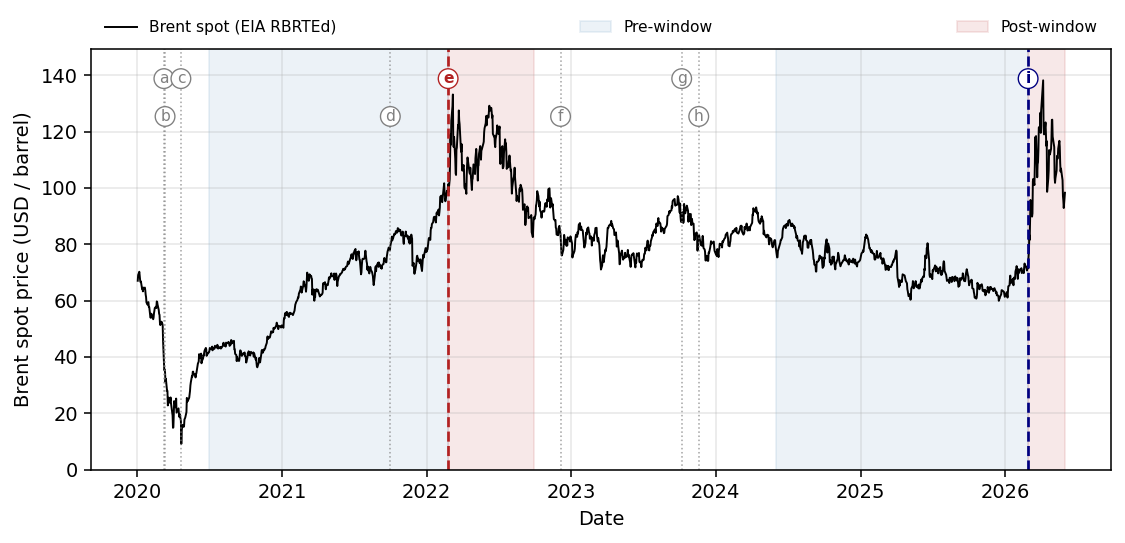
\includegraphics[width=0.92\textwidth]{figures/brent_timeline.png}
\caption{Brent crude spot price, 2020--2026, with the two focal event dates. Brent
roughly doubled after both shocks from a similar $\sim$\$75 base, but from very
different pre-event trajectories: a steep 2020--22 recovery rally before Russia, and a
mild net decline through 2024--25 before Hormuz. This trajectory asymmetry is what makes
a na\"ive trend-extrapolation counterfactual unreliable (Section~\ref{sec:results}).}
\label{fig:timeline}
\end{figure}

The two pre-windows differ in a way that matters later. The Russia pre-period is
volatile (SD~\$16.4, spanning the COVID recovery and the 2021 reflation rally); the
Hormuz pre-period is much calmer (SD~\$6.6). This difference drives much of the
contrast in the two events' inference: a volatile pre-period widens the placebo
distribution and weakens Russia's permutation test, even though its magnitude is
well-documented.

% ===================================================================
\section{Empirical Strategy and Validation}\label{sec:methods}
% ===================================================================
\subsection{Estimators}
All five estimators (Table~\ref{tab:models}) take the same input (log donor levels) and
target log Brent over the pre-window, then project the post-window counterfactual.
\emph{Convex SCM} solves the classic nested optimisation: non-negative weights summing
to one, chosen to minimise pre-period RMSPE \citep{abadie2010}. \emph{Augmented SCM}
adds a ridge penalty that corrects for imperfect pre-fit and allows limited
extrapolation \citep{benmichael2021}. The \emph{elastic net} relaxes the simplex to
signed, sparse coefficients \citep{zouhastie2005,doudchenko2016}. \emph{XGBoost} fits
shallow gradient-boosted trees \citep{chenguestrin2016}, deliberately constrained
(depth-2 stumps, strong regularisation, row/column subsampling) for the small-sample
regime. \emph{Bayesian ridge} is a conjugate Bayesian linear regression on donor levels,
the regression component of BSTS \citep{brodersen2015}. Hyperparameters are tuned over
small grids (3--9 configurations) to bound the selection bias of \citet{cawley2010}; the
convex SCM has no tuned hyperparameter. We implement the pipeline in Python: the convex
and augmented SCM solvers are written directly on top of \texttt{numpy}/\texttt{scipy},
the elastic net and Bayesian ridge come from \texttt{scikit-learn}, gradient boosting
from \texttt{xgboost}, and the ARIMA baselines and structural-break statistics from
\texttt{statsmodels} plus our own implementations of the Bai--Perron and
Harvey--Leybourne--Taylor tests.

\subsection{Donor cleanliness battery}
Before any model is fit, each donor's own return series is tested for a mean shift at
$T_0$ using a permutation form of the known-break test of \citet{chow1960} (rather than
the unknown-break test of \citet{andrews1993}, since the date is known), together with a
Wilcoxon event-window test \citep{brownwarner1985}; a donor is flagged if either rejects
after Benjamini--Hochberg FDR control \citep{benjaminihochberg1995}. Regime stability is
checked with distance correlation across pre-period thirds \citep{szekely2007} and with
Bai--Perron break dating \citep{baiperron1998,baiperron2003}; an I(0)/I(1)-robust
trend-break test \citep{harvey2009,kpss1992} confirms no donor's own trend breaks at
either $T_0$. Empirically, for Hormuz 31 of 32 donors agree between audit and tests
(only Cotton differs); for Russia the tests confirm the broad picture and add one flag
(CNY) attributable to concurrent China dynamics, not the war.

\subsection{Validation battery and its logic}
A credible SCM estimate must clear three levels: pre-event fit, donor identification,
and inference \citep{abadie2021}. We run, per model and event: (a) expanding-window
walk-forward cross-validation for out-of-sample fit \citep{hyndman2018,bergmeir2012};
(b) the in-space placebo, refitting each donor as a placebo treated unit and ranking
Brent's post/pre RMSPE ratio against the resulting distribution \citep{abadie2010},
reading the permutation $p$-value with the symmetry caveat of \citet{hahnshi2017};
(c) the in-time placebo at a fake $T_0$ six months early, formalised as the mixed
placebo test of \citet{chenyan2023}; (d) leave-one-donor-out; (e) the cross-event weight
transfer; (f) a deliberately contaminated set of na\"ive univariate counterfactuals
(random walk, drift, linear trend, frozen ARIMA) as a floor; and (g) the signed
contamination-bias diagnostic of equation~\eqref{eq:bias}. Following
\citet{roth2022,rambachanroth2023}, pre-period diagnostics are reported and interpreted
rather than turned into pass/fail thresholds; flagged models are \emph{not} auto-excluded,
because the cross-model IQR is itself the model-uncertainty band.

The headline per event is the cross-model \emph{median} gap, with the IQR as the band.
Where a model's pre-period gap series trends, we report a drift adjustment: a slope of
$\hat\beta$\,\%/yr over a post-window of $L$ years contributes $\hat\beta L$ percentage
points independent of treatment, so the drift-adjusted gap subtracts it.

% ===================================================================
\section{Results}\label{sec:results}
% ===================================================================
\subsection{Pre-event fit}
Table~\ref{tab:wfcv} reports walk-forward CV. For Hormuz, four of five models clear the
heuristic flag (validation/training RMSE ratio below~2); only Bayesian ridge, at 2.28,
is flagged. For Russia, two of five clear it (convex SCM and elastic net); with VIX kept
in the pool the augmented SCM rises just past the threshold (2.06), and XGBoost (3.24)
and Bayesian ridge (3.09) fail more clearly. The flags are not exclusions: they identify
which models to read with caution, and the most flagged model (Bayesian ridge) is the one
whose headline gap is the ensemble outlier.

\begin{table}[h]
\centering
\caption{Walk-forward cross-validation (5 expanding folds, 20-day horizons). A
validation/training RMSE ratio above 2 is a heuristic overfit flag, not an exclusion rule.}
\label{tab:wfcv}
\small
\begin{tabular}{@{}llrrrl@{}}
\toprule
Event & Model & train RMSE & val RMSE & val/train & Flag \\
\midrule
Russia & Convex SCM     & 0.113 & 0.141 & 1.25 & OK \\
Russia & Augmented SCM  & 0.046 & 0.095 & 2.06 & overfit \\
Russia & Elastic net    & 0.051 & 0.102 & 1.99 & OK \\
Russia & XGBoost        & 0.039 & 0.127 & 3.24 & overfit \\
Russia & Bayesian ridge & 0.034 & 0.105 & 3.09 & overfit \\
\addlinespace
Hormuz & Convex SCM     & 0.060 & 0.083 & 1.40 & OK \\
Hormuz & Augmented SCM  & 0.049 & 0.075 & 1.54 & OK \\
Hormuz & Elastic net    & 0.052 & 0.079 & 1.51 & OK \\
Hormuz & XGBoost        & 0.044 & 0.082 & 1.84 & OK \\
Hormuz & Bayesian ridge & 0.034 & 0.078 & 2.28 & overfit \\
\bottomrule
\end{tabular}
\end{table}

\subsection{Headline estimates}
Table~\ref{tab:headline} reports the per-model post-window gap, the drift contribution,
and the drift-adjusted gap, for both events; Figure~\ref{fig:paths} plots the observed
and synthetic paths. \textbf{Russia 2022} yields an ensemble-median premium of
\SI{22.0}{\percent} over the seven-month window (IQR \SIrange{10.9}{30.8}{\percent}),
with an implied counterfactual mean of \$88.6/bbl against an actual \$108.5. This is
consistent with the documented \$95$\to$\$130 move and its partial reversion by
September. \textbf{Hormuz 2026} yields an ensemble-median premium of
\SI{55.9}{\percent} over the window to mid-June (IQR \SIrange{51.2}{56.6}{\percent}),
with an actual post-window mean of \$106.9 against an implied counterfactual of
$\sim$\$68.6. The Hormuz IQR is far tighter than Russia's ($\sim$5 vs $\sim$20 pp),
reflecting the calmer Hormuz pre-period.

\begin{table}[h]
\centering
\caption{Headline post-event gaps (\%). Drift-adjusted $=$ raw $-$ drift contribution.
Ensemble $=$ cross-model median; band $=$ IQR (Q25--Q75).}
\label{tab:headline}
\small
\begin{tabular}{@{}lrrr@{\hskip 1.2em}rrr@{}}
\toprule
& \multicolumn{3}{c}{Russia 2022 (7 mo)} & \multicolumn{3}{c}{Hormuz 2026 ($\sim$3.5 mo)}\\
\cmidrule(lr){2-4}\cmidrule(lr){5-7}
Model & Raw & Drift & Adj. & Raw & Drift & Adj. \\
\midrule
Convex SCM     & 33.6 & $+5.2$ & 28.4 & 55.9 & $-1.4$ & 57.3 \\
Augmented SCM  & 10.9 & $+0.3$ & 10.6 & 56.8 & $-0.4$ & 57.1 \\
Elastic net    & 22.0 & $+0.7$ & 21.2 & 56.6 & $-0.8$ & 57.4 \\
XGBoost        & 30.8 & $+1.8$ & 28.9 & 51.2 & $-1.5$ & 52.7 \\
Bayesian ridge & $-9.0$ & $+0.1$ & $-9.1$ & 43.0 & $-0.0$ & 43.0 \\
\midrule
\textbf{Ensemble median} & \textbf{22.0} & n/a & \textbf{21.2} & \textbf{55.9} & n/a & \textbf{57.1} \\
\textbf{IQR} & \textbf{[10.9, 30.8]} & n/a & n/a & \textbf{[51.2, 56.6]} & n/a & n/a \\
\bottomrule
\end{tabular}
\end{table}

\begin{figure}[h]
\centering
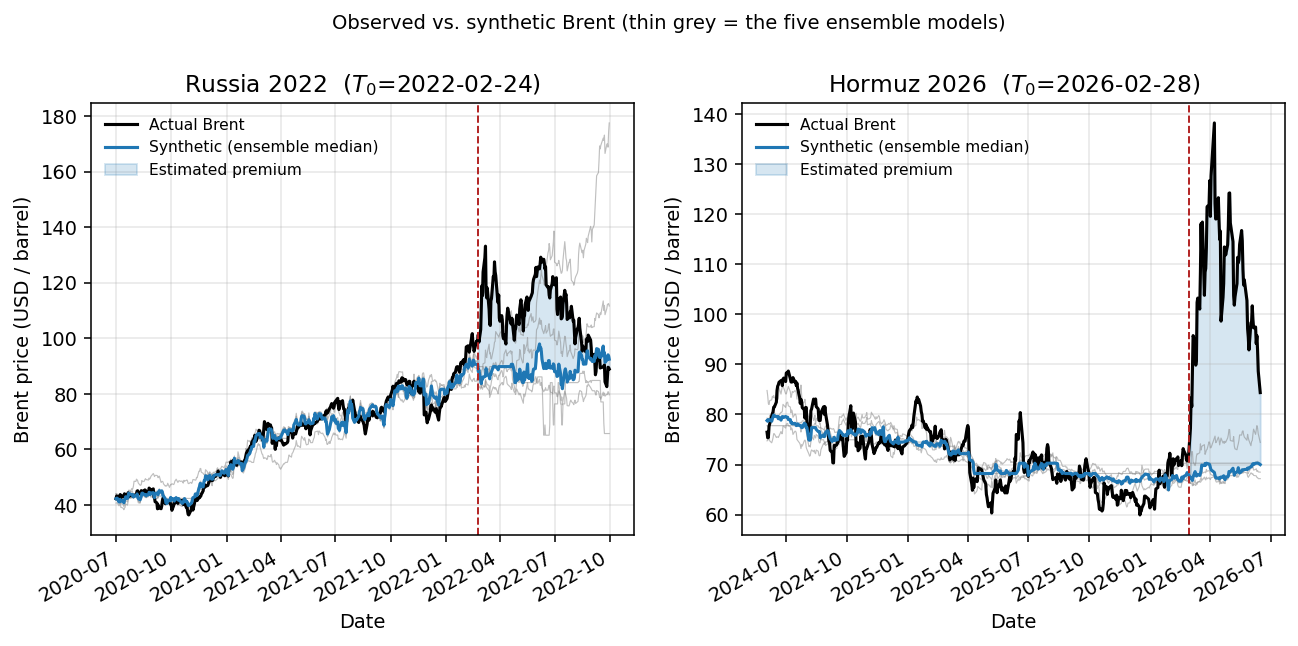
\includegraphics[width=\textwidth]{figures/counterfactual_paths.png}
\caption{Observed Brent (black) vs.\ the synthetic counterfactual. The thick blue line
is the ensemble-median synthetic; thin grey lines are the five individual models; the
shaded region after $T_0$ (dashed red) is the estimated premium. The synthetics track
Brent closely pre-event and decouple sharply afterward.}
\label{fig:paths}
\end{figure}

\paragraph{Economic reading of the model spread.} The cross-model dispersion has an
economic explanation rather than being noise. Convex SCM, confined to the simplex,
leans on the most stable donors (the FX block) as a ``trend baseline'' and adds
soft-commodity deltas (Coffee, Sugar for Russia). The Bayesian ridge, with
unconstrained Gaussian coefficients, loads heavily and with large opposing signs on
currencies; for Russia those currencies were pushed around by the simultaneous,
historically large Fed tightening cycle, a macro factor orthogonal to the invasion.
That is why Bayesian ridge is the Russia outlier (a negative full-window gap) and why
it earns the highest walk-forward overfit flag: it is the expected behaviour of an
unregularised linear model in a pre-period with a strong non-event macro driver, and it
is the reason the ensemble uses the \emph{median} rather than the mean. For Hormuz,
whose calmer pre-period lacks an analogous confound, the five models agree to within
$\sim$5 pp.

\subsection{Inference: the in-space placebo}
Table~\ref{tab:placebo} and Figure~\ref{fig:placebo} report the in-space placebo. For
\textbf{Hormuz}, Brent ranks \emph{first} among all placebo units under every model and
both pools, with a post/pre RMSPE ratio (6.9--10.2) above every donor's, so the
permutation $p$-value sits at the attainable floor (0.050 in the 19-donor pool, 0.030 in
the 32-donor pool). This is the strongest signal the test can give at this sample size.
For \textbf{Russia}, no model reaches the floor (XGBoost comes closest at $p=0.20$ in the
19-donor pool, $0.15$ in the 32-donor pool); the
volatile 2020--22 pre-period gives donors large pre-period RMSPE too, widening the placebo
distribution. This is a known low-power property of the in-space placebo at volatile
pre-periods \citep{abadie2010}, not evidence of a small effect. Russia's magnitude is
independently documented and externally validated below.

\begin{table}[h]
\centering
\caption{In-space placebo permutation $p$-values and Brent's post/pre RMSPE ratio
(19-donor pool). Floor $=1/(N{+}1)$: 0.050 (19-donor), 0.030 (32-donor).}
\label{tab:placebo}
\small
\begin{tabular}{@{}llrrr@{}}
\toprule
Event & Model & $p$ (19-donor) & $p$ (32-donor) & Brent ratio \\
\midrule
Russia & Convex SCM     & 0.50 & 0.50 & 2.75 \\
Russia & Augmented SCM  & 0.60 & 0.47 & 3.51 \\
Russia & Elastic net    & 0.40 & 0.41 & 4.08 \\
Russia & XGBoost        & 0.20 & 0.15 & 7.75 \\
Russia & Bayesian ridge & 0.60 & 0.53 & 5.88 \\
\addlinespace
Hormuz & Convex SCM     & \textbf{0.050} & \textbf{0.029} & 6.93 \\
Hormuz & Augmented SCM  & \textbf{0.050} & \textbf{0.029} & 8.45 \\
Hormuz & Elastic net    & \textbf{0.050} & \textbf{0.029} & 8.53 \\
Hormuz & XGBoost        & \textbf{0.050} & \textbf{0.029} & 10.19 \\
Hormuz & Bayesian ridge & \textbf{0.050} & \textbf{0.029} & 10.24 \\
\bottomrule
\end{tabular}
\end{table}

\begin{figure}[h]
\centering
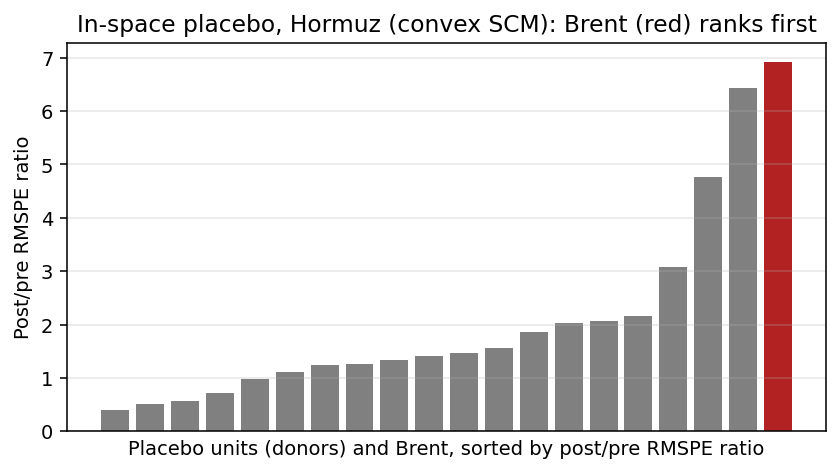
\includegraphics[width=0.72\textwidth]{figures/placebo_hormuz.png}
\caption{In-space placebo for Hormuz (convex SCM). Each bar is one unit's post/pre RMSPE
ratio; Brent (red) is the largest, ranking first among all 19 placebo units, so the
permutation test rejects at the attainable floor.}
\label{fig:placebo}
\end{figure}

\subsection{Robustness}
\paragraph{Russia magnitude / external validation.} Because Russia is a known event, we
validate its magnitude against the EIA's last two \emph{pre-invasion} Short-Term Energy
Outlook forecasts (issued before 24 February 2022), which are an independent structural
counterfactual sharing no information path with the SCM. Over the identical 151-day
window, the ensemble-median synthetic mean (\$88.6) sits within \$3.6 of the STEO Feb-2022
forecast (\$84.9); three of five models bracket the STEO anchor to within $\pm$\$4. Two
independent methods agreeing on the counterfactual is strong evidence the SCM is not
producing an implausible path.

\paragraph{Post-window horizon sensitivity.} Figure~\ref{fig:sensitivity} reports the gap
at 1/2/3/6-month and full horizons. The two events show opposite, diagnostic profiles.
Russia \emph{declines} with horizon (31\%~$\to$~22\%): the signature of delayed
contamination, as second-round war channels switch on through 2022 and pull the synthetic
up, so the full-window figure is conservative and the least-contaminated one-month
estimate is $\sim$31\%. Hormuz \emph{rises then eases} (46\%~$\to$~59\%~$\to$~56\%): the
chokepoint premium builds in and holds, the opposite of attenuation; the slight easing to
56\% at the full horizon reflects Brent's partial mid-June pullback, captured by extending
the window to the latest data. That the same diagnostic declines for Russia and rises for
Hormuz shows it is not a mechanical artefact.

\begin{figure}[h]
\centering

\includegraphics[width=0.78\textwidth]{figures/postwindow_sensitivity.png}
\caption{Ensemble-median gap by post-event horizon (shaded $=$ IQR across models). Russia
attenuates with horizon (delayed-contamination signature); Hormuz rises then plateaus
(the premium builds in and holds).}
\label{fig:sensitivity}
\end{figure}

\paragraph{Leave-one-donor-out.} Dropping each weighted donor in turn leaves the Hormuz
estimate tight around its baseline (convex 51.2--59.3, ASCM 54.6--60.5, elastic 55.2--62.2,
XGBoost 51.6--57.7\%); no single donor drives the result. Russia is wider (e.g.\ convex
32.8--59.6\%), consistent with its volatile pre-period and the simplex's reliance on a few
soft-commodity donors.

\paragraph{Cross-event weight transfer.} Applying Russia-fitted weights to the Hormuz
window (Table~\ref{tab:transfer}), convex SCM is the only model that transfers to a clearly
\emph{positive} Hormuz premium (25.3\%) with a degraded but non-pathological pre-fit
(pre-RMSPE 5$\times$ independent); the augmented SCM transfers to roughly zero ($-0.8$\%,
7$\times$), and the signed-regression, tree, and prior-dominated models go strongly negative
with pre-RMSPE 14--280$\times$ independent. We therefore read the transfer as weak,
convex-only corroboration that \emph{some} positive premium survives a change of regime,
not as confirmation of its level: the headline magnitude rests on the within-event ensemble.
Once the window is extended through Brent's June pullback, the regime gap between the
2020--22 and 2024--26 factor structures is evidently wider than over the shorter window.

\begin{table}[h]
\centering
\caption{Cross-event weight transfer: Russia-fitted weights applied to Hormuz. Independent
and transferred pre-period RMSPE in log units.}
\label{tab:transfer}
\small
\begin{tabular}{@{}lrrrr@{}}
\toprule
Model & Indep.\ gap (\%) & Transf.\ gap (\%) & Indep.\ RMSPE & Transf.\ RMSPE \\
\midrule
Convex SCM     & 55.9 & 25.3   & 0.066 & 0.336 \\
Augmented SCM  & 56.8 & $-0.8$  & 0.066 & 0.467 \\
Elastic net    & 56.6 & $-68.6$ & 0.054 & 1.513 \\
XGBoost        & 51.2 & $-44.1$ & 0.053 & 0.928 \\
Bayesian ridge & 43.0 & $-100.0$ & 0.037 & 18.567 \\
\bottomrule
\end{tabular}
\end{table}

\paragraph{Na\"ive counterfactual floor.} Against donor-free univariate counterfactuals
(Table~\ref{tab:naive}), the SCM adds value, and the na\"ive methods' bias \emph{flips
sign across events} purely because the pre-window trend sign differs. A linear trend
extrapolates Russia's recovery rally upward and returns an implausible \emph{negative}
full-window gap ($-4\%$), but extrapolates Hormuz's mild downtrend and \emph{inflates} the
gap to 71\%. The trend-free random-walk null gives Russia $+8.7\%$ and Hormuz $+48.9\%$,
with the SCM $\sim$13 and $\sim$7 pp above respectively. The SCM, anchored to donor
co-movement rather than Brent's own momentum, is far more stable across the two regimes,
which is the concrete demonstration of why a donor-based counterfactual is necessary.

\begin{table}[h]
\centering
\caption{SCM vs.\ na\"ive univariate counterfactuals, full-window gap (\%). RW flat/drift:
random-walk carry / with drift; Lin.\ trend: linear pre-trend extrapolation; ARIMA rw/mr:
frozen AR(1) forecasts (random-walk / mean-reverting).}
\label{tab:naive}
\small
\begin{tabular}{@{}lrrrrrr@{}}
\toprule
Event & SCM median & RW flat & RW drift & Lin.\ trend & ARIMA rw & ARIMA mr \\
\midrule
Russia & 22.0 & 8.7  & $-6.9$ & $-4.2$ & 9.2  & 26.5 \\
Hormuz & 55.9 & 48.9 & 49.8   & 70.9   & 48.1 & 48.7 \\
\bottomrule
\end{tabular}
\end{table}

\paragraph{Sign of the contamination bias.} Using equation~\eqref{eq:bias} with a
Brent-free common factor, we sign the bias per (linear) model. For \textbf{Hormuz} the
full-window bias is small and \emph{negative} (conservative) for all four linear models
($-1.3$ to $-7.6$\%), so the large premium is not a contamination artefact. For
\textbf{Russia} the full-window bias is large and \emph{positive} (overestimate, +13 to
+21\% for three of four models), concentrated in low-reliability soft commodities whose
2022 idiosyncratic drift the convex/elastic fits leaned on; following the reliability logic
of \citet{hammiratrix2024}, splitting donors by pre-window factor $R^2$ shows the bias sits
mostly in the low-$R^2$ (unreliable) donors. The asymmetric conclusion is that
contamination is conservative for the focal Hormuz estimate but inflates the Russia
\emph{full-window} number; Russia's magnitude validation therefore rests on the early/peak
window (where the \$95$\to$\$130 move is recovered), not on the attenuated full-window
average.

\subsection{Interpretation}
Our estimate places the 2026 Hormuz chokepoint premium at roughly \SI{56}{\percent} of
Brent's no-event level over the first $\sim$3.5 months. The number holds up across all five
estimators and across the checks we ran: the in-space placebo reaches its floor,
leave-one-out stays tight, the contamination bias is conservative, and the SCM clears
the na\"ive baselines. The cross-event transfer is the weakest of the checks: only convex
SCM transfers to a clearly positive premium, so we lean on it for the sign rather than the
level. We read the estimate as a complement to, not a competitor of, the
structural scenario estimates from energy institutions: those answer ``what price does
an assumed barrel shortfall imply,'' while the SCM answers ``what price gap does the
observed cross-asset co-movement imply.''
For the policy levers of Section~\ref{sec:lit} (reserve releases, monetary pass-through,
fiscal buffers), the integrated, path-level premium is the relevant input, and the
estimate here provides it with an auditable identification argument.

% ===================================================================
\section{Conclusion}\label{sec:conclusion}
% ===================================================================
We estimated the Brent-price effect of the 2026 Strait of Hormuz disruption by building a
counterfactual with an ensemble synthetic control, validating the design first on the known
Russia 2022 event. Over the window to mid-June 2026 the ensemble-median premium is
$\sim$56\% (IQR 51--57\%), large and positive under every estimator, and it survives the
in-space placebo (Brent first among all units, $p$ at the floor), leave-one-out, the
contamination-bias sign check, and the na\"ive-baseline comparison; the cross-event transfer
gives weaker, convex-only support for a positive premium. On the calibration event the same
machinery recovers a magnitude consistent with the documented \$95$\to$\$130 move and within
\$3.6/bbl of the EIA's pre-invasion structural forecast.

The estimate's value is as a reduced-form, data-driven complement to structural scenario
analysis, with an identification argument a reviewer can audit donor by donor. Several
limitations qualify it. The Hormuz post-window is short ($\sim$72 observations), so every
inference test is under-powered and the placebo can only reach its floor; the convex
synthetic under-represents Brent's volatility, which the augmented SCM corrects; the
cross-event transfer degrades once the window is extended through Brent's June pullback;
the Bayesian-ridge model is a regression proxy for BSTS, not the full state-space model;
and the estimand is a reduced-form total effect, not a supply/demand/risk decomposition.
Natural extensions are a longer post-window as data accrue, per-donor
delayed-contamination onset dating to sharpen the post-window choice, and a full BSTS
implementation for autocorrelation-aware credible intervals. None of these changes the
central finding: the observed co-movement of global markets with Brent implies that the
2026 Hormuz disruption added a large, statistically distinguishable premium to crude, on
the order of half its no-event price.

\bibliography{references}

\appendix
% ===================================================================
\section{Robustness grid}\label{app:grid}
% ===================================================================
The headline uses the preferred specification (shared 19-donor pool, preferred pre-window,
ensemble median). The full grid varies (i) the pre-window (preferred, extended, and narrow
specifications); (ii) the donor pool (shared 19, permissive 26 for Russia, full 32); and
(iii) the model (each of the five plus the median). For Russia the donor-pool sweep is
itself a diagnostic: the gap is expected to \emph{shrink} monotonically from the clean
19-donor pool to the contaminated 32-donor pool, because Russia-treated donors get inflated
by the same shock and pull the synthetic up. If this monotonic pattern holds, the
SUTVA-driven exclusion logic is empirically supported.

% ===================================================================
\section{Bayesian ridge and full BSTS}\label{app:bsts}
% ===================================================================
The fifth ensemble member implements only the regression-on-donors term $\beta'x_t$ of the
Bayesian structural time-series model of \citet{brodersen2015}, with a conjugate
Gaussian--Gamma prior. It omits the local-linear \emph{trend}, the \emph{seasonal}
component, the \emph{spike-and-slab} donor selection, and the autocorrelation-aware
posterior over the full state trajectory. At our sample size, with no strong weekly
seasonality in daily oil prices, the regression term carries most of the signal, so the
proxy is an adequate Bayesian-flavoured diversifier; but its credible intervals are Gaussian
and ignore autocorrelation, and its donor ``importances'' are standardised-coefficient
magnitudes, not true posterior inclusion probabilities. We therefore call it a Bayesian
ridge regression rather than a BSTS, and read its placebo $p$-values as rank statistics
rather than formal probabilities (Table~\ref{tab:placebo}). A full BSTS implementation is the
natural route to autocorrelation-aware credible intervals in a future iteration.

% ===================================================================
\section{Structural-break tests}\label{app:breaks}
% ===================================================================
Two break tests support donor screening. \emph{Bai--Perron}
\citep{baiperron1998,baiperron2003} dates breaks in the donor--Brent weekly-return
relationship $r^{\text{donor}}_t=\alpha_s+\beta_s r^{\text{Brent}}_t+\varepsilon_t$ by
globally minimising segment SSR via dynamic programming, with the break count chosen by BIC.
Only VIX shows a break strictly inside a pre-window (2022-01-07). We treat the break tests as
informative rather than automatically disqualifying: the VIX break is a loading-stability
signal, it does not reproduce on the analysis window alone, and the in/out sensitivity is
below 1 pp, so VIX is retained (Section~\ref{sec:data}). The relationship specification is
Brent-based, so a break \emph{at} $T_0$ is ambiguous; the
complementary \citet{harvey2009} trend-break test resolves this by testing the donor's
\emph{own} log-level trend with a statistic whose asymptotic size is invariant to whether the
series is I(0) or I(1): it weights an I(0)-optimal and an I(1)-optimal sup-$t$ statistic by
KPSS stationarity weights \citep{kpss1992}. Empirically all 32 donors are classified I(1)-like
and none rejects a trend break within $\pm$8 weeks of either $T_0$, so no retained donor was
itself trend-treated by either event.

\end{document}
